%----------------------------------------------------------------------------------
% Exemplo do uso da classe tcc.cls. Veja o arquivo .cls
% para mais detalhes e instruções.
%----------------------------------------------------------------------------------

% Seleção de idioma da monografia. Por enquanto as únicas opções
% suportadas são 'portuguese' e 'english'
% Para impressão em frente e verso, use a opção 'twoside'. Da
% mesma forma, use 'oneside' para impressão em um lado apenas.
\documentclass[portuguese,oneside]{tcc}

%----------------------------------------------------------------
% Coloque seus pacotes abaixo.
%
% Obs.: muitos pacotes de uso comum do LaTeX, como amsmath,
% geometry e url já são automaticamente incluídos pela classe
% (veja o arquivo .cls). Isso torna obrigatória a presença destes
% no sistema para o uso desta classe, mas ao mesmo tempo o uso se
% torna mais simples.  Recomendo a instalação da versão mais
% recente da distribuição TeXLive (para Windows e UNIXes):
% www.tug.org/texlive/
%
% Pacotes e opções já incluídas automaticamente:
%
% \RequirePackage[T1]{fontenc}[2005/09/27]
% \RequirePackage[utf8x]{inputenc}[2008/03/30]
% \RequirePackage[english,brazil]{babel}[2008/07/06]
% \RequirePackage[a4paper]{geometry}[2010/09/12]
% \RequirePackage{textcomp}[2005/09/27]
% \RequirePackage{lmodern}[2009/10/30]
% \RequirePackage{indentfirst}[1995/11/23]
% \RequirePackage{setspace}[2000/12/01]
% \RequirePackage{textcase}[2004/10/07]
% \RequirePackage{float}[2001/11/08]
% \RequirePackage{amsmath}[2000/07/18]
% \RequirePackage{amssymb}[2009/06/22]
% \RequirePackage{amsfonts}[2009/06/22]
% \RequirePackage{url}
% \RequirePackage[table]{xcolor}[2007/01/21]
%----------------------------------------------------------------
% Para inserção de figuras.
\usepackage{graphicx}
% Utilize a opção 'pdftex' se você estiver usando o pdflatex (que
% permite figuras em formatos como .jpg ou .png)
%\usepackage[pdftex]{graphicx}

% Para tabelas com elementos ocupando mais de uma linha
\usepackage{multirow}
% Para frações na mesma linha (ex. ⅓).
\usepackage{nicefrac}
% Para inserir figuras lado a lado.
% \usepackage{subfigure}
% Para formatar algoritmos.
% A opção [algo2e] é necessária para evitar conflitos
% com as definições da classe.
%\usepackage[algo2e]{algorithm2e}
\usepackage{algorithmic}
% Um float do tipo algoritmo. No momento
% este pacote é incompatível com a classe.
%\usepackage{algorithm}
\usepackage{enumitem}
\usepackage{booktabs}  % tabelas com filetes horizontais
\usepackage{tabularx}  % colunas de largura automática
\usepackage{pdflscape} % páginas em paisagem
\usepackage{afterpage}  % adia a tabela em paisagem para a próxima página
\usepackage{pgfgantt}  % cronograma em formato de Gantt
\definecolor{ganttBar}{HTML}{3A7BD5}

% Listagens de código com as cores do tema Light Modern do VS Code
\usepackage{listings}
\definecolor{vscText}{HTML}{3B3B3B}
\definecolor{vscKeyword}{HTML}{0000FF}
\definecolor{vscVariable}{HTML}{001080}
\definecolor{vscNumber}{HTML}{098658}
\definecolor{vscComment}{HTML}{008000}
\definecolor{vscLabel}{HTML}{795E26}
\definecolor{vscFrame}{HTML}{E5E5E5}
\definecolor{vscBack}{HTML}{F8F8F8}
\newcommand{\asmnum}[1]{\textcolor{vscNumber}{#1}}
\newcommand{\asmlabel}[1]{\textcolor{vscLabel}{#1}}
\lstdefinelanguage{riscv}{
    morekeywords={add,addi,sub,and,andi,or,ori,xor,xori,sll,slli,srl,srli,sra,srai,slt,slti,sltu,sltiu,lui,auipc,lb,lbu,lh,lhu,lw,sb,sh,sw,mul,mulh,mulhu,mulhsu,div,divu,rem,remu,beq,bne,blt,bge,bltu,bgeu,beqz,bnez,j,jal,jalr,jr,ret,li,la,mv,nop,ecall,ebreak,mret,csrr,csrw,csrs,csrc,csrrw,csrrs,csrrc,csrsi,csrci,csrwi},
    morekeywords=[2]{x0,x1,x2,x3,x4,x5,x6,x7,x8,x9,x10,x11,x12,x13,x14,x15,x16,x17,x18,x19,x20,x21,x22,x23,x24,x25,x26,x27,x28,x29,x30,x31,mie,mip,mstatus,mepc,mcause,mtvec,mscratch},
    morecomment=[l]{\#},
    sensitive=true,
}
\lstdefinestyle{vscodelight}{
    language=riscv,
    basicstyle=\ttfamily\small\color{vscText},
    keywordstyle=\color{vscKeyword},
    keywordstyle=[2]\color{vscVariable},
    commentstyle=\color{vscComment},
    backgroundcolor=\color{vscBack},
    frame=single,
    rulecolor=\color{vscFrame},
    framesep=6pt,
    xleftmargin=6pt,
    xrightmargin=6pt,
    columns=fullflexible,
    keepspaces=true,
    showstringspaces=false,
    escapeinside={(*}{*)},
    extendedchars=true,
    literate={á}{{\'a}}1 {é}{{\'e}}1 {í}{{\'i}}1 {ó}{{\'o}}1 {ú}{{\'u}}1
             {ã}{{\~a}}1 {õ}{{\~o}}1 {ç}{{\c{c}}}1 {â}{{\^a}}1 {ê}{{\^e}}1
             {ô}{{\^o}}1 {à}{{\`a}}1,
}

%%%%%%%%%%%%%%%%%%%%%%%%%%%%%%%%%%%%%%%%%%%%%
%% Angelo: Pacotes para config de referencias
\usepackage[authoryear]{natbib}
\usepackage[colorlinks=true,linkcolor=blue,citecolor=blue,urlcolor=blue]{hyperref}
\usepackage[brazilian]{cleveref}
\newlist{objetivos}{enumerate}{1}
\setlist[objetivos]{label=O\arabic*., ref=O\arabic*}
\crefname{objetivosi}{objetivo}{objetivos}
\Crefname{objetivosi}{Objetivo}{Objetivos}
\newlist{atividades}{enumerate}{1}
\setlist[atividades]{label=A\arabic*., ref=A\arabic*}
\crefname{atividadesi}{atividade}{atividades}
\Crefname{atividadesi}{Atividade}{Atividades}
%%%%%%%%%%%%%%%%%%%%%%%%%%%%%%%%%%%%%%%%%%%%%

%%%%%%%%%%%%%%%%%%%%%%%%%
%%%% Remover para entrega
\usepackage{soul}
%%%%%%%%%%%%%%%%%%%%%%%%%


%----------------------------------------------------------------
% Autor (OBRIGATÓRIO)
%----------------------------------------------------------------
\author{Pedro Fam Haggstram}

%----------------------------------------------------------------
% Título (OBRIGATÓRIO). Devem ser passados DOIS parâmetros,
% o título em português E o inglês, não importando o idioma
% escolhido. Os títulos são utilizados para a montagem da capa,
% resumo e abstract mais tarde.
%----------------------------------------------------------------
\title{Fuzzing Baseado em Kernels de Aplicação para a Verificação Funcional de um Processador RISC-V Parametrizável}
      {Application-Kernel-Based Fuzzing for the Functional Verification of a Configurable RISC-V Processor}

%----------------------------------------------------------------
% Opções para o tipo de trabalho (OBRIGATÓRIO)
%----------------------------------------------------------------
\tipotrabalho{\ptci}         % Proposta de Trabalho de Conclusão
%\tipotrabalho{\tci}         % Trabalho de Conclusão I
%\tipotrabalho{\tcii}        % Trabalho de Conclusão II

%----------------------------------------------------------------
% Seleção do curso ("este trabalho é um requisito parcial para
% obtenção do grau de (mestre ou doutor) em Ciência da Computação").
%----------------------------------------------------------------
\curso{\cc} % Ciência da Computação
%\curso{\si} % Sistemas de Informação
%\curso{\es} % Engenharia de Software

%----------------------------------------------------------------
% Orientador (e Co-orientador, caso haja um). É OBRIGATÓRIO
% informar pelo menos o orientador.
%----------------------------------------------------------------
\orientador{Angelo Elias Dal Zotto}

%----------------------------------------------------------------
% A capa é inserida automaticamente. Por isso não é necessário
% chamar \maketitle
%----------------------------------------------------------------
\begin{document}

%----------------------------------------------------------------
% Depois da capa vem a dedicatória e a epígrafe. Apenas na entrega final
%----------------------------------------------------------------
% \dedicatoria{Dedico este trabalho a Manuela.}

% \epigrafe{The art of simplicity is a puzzle of complexity.}
%          {Douglas Horton}

%----------------------------------------------------------------
% Também dá para fazer as duas na mesma página:
%----------------------------------------------------------------
%\dedigrafe{Dedico este trabalho a meus pais.}
%          {The art of simplicity is a puzzle of complexity.}
%          {Douglas Horton}

%----------------------------------------------------------------
% A seguir, a página de agradecimentos (OPCIONAL):
%----------------------------------------------------------------
% \begin{agradecimentos}
% À lorem ipsum, dolor sit amet consetetur sadipscing elitr sed diam
% nonumy eirmod tempor. invidunt ut labore et dolore magna aliquyam

% À erad sed, diam voluptua at vero, eos et accusam et justo duo
% dolores et ea rebum stet clita.

% À kasd gubergren, no sea. takimata sanctus est lorem ipsum dolor sit
% amet lorem ipsum dolor sit amet. consetetur sadipscing elitr sed

% À diam nonumy, eirmod tempor, invidunt ut labore et dolore magna
% aliquyam erat sed diam voluptua at.
% \end{agradecimentos}

%----------------------------------------------------------------
% Resumo, com as palavras-chave passadas por parâmetro
% (OBRIGATÓRIO, ao menos para teses e dissertações)
%----------------------------------------------------------------
\begin{resumo}{verificação funcional, \textit{fuzzing}, RISC-V, RS5, RISCOF}
A verificação funcional de processadores depende de programas de teste capazes de exercitar as interações entre as instruções e os mecanismos internos da microarquitetura. O RS5, um processador RISC-V de 32 bits parametrizável, é validado pela suíte \textit{riscv-tests} e pelos testes arquiteturais do RISCOF, ambos limitados a cenários escritos manualmente. Este trabalho propõe um \textit{fuzzer} para o RS5 construído sobre o RISCOF. Ele gera programas pela combinação e mutação de blocos de Assembly extraídos de aplicações reais, executa-os em diferentes configurações do processador e compara as assinaturas produzidas pelo RS5, simulado com o Verilator, com as do modelo de referência Sail. A exploração é orientada por realimentação extraída do estado interno do processador. Como trabalho prévio, foram construídos um gerador preliminar e a infraestrutura de \textit{fuzzing}, usados para comparar fontes de realimentação em cerca de 1,8 milhão de programas. As arestas entre estados do \textit{pipeline} não saturaram em 200.000 programas, enquanto a cobertura de código do Verilator se esgotou em algumas centenas. Com o gerador preliminar, a exploração guiada não superou a geração aleatória, o que direciona as próximas etapas para o corpus de blocos e para os operadores de mutação. O estudo também revelou uma divergência entre o RS5 e o Sail no tratamento de interrupções. Por fim, é apresentado o cronograma das atividades restantes.
\end{resumo}

%----------------------------------------------------------------
% Abstract, com as palavras-chave passadas por parâmetro
% (OBRIGATÓRIO, ao menos para teses e dissertações)
%----------------------------------------------------------------
\begin{abstract}{functional verification, fuzzing, RISC-V, RS5, RISCOF}
Functional verification of processors depends on test programs that exercise the interactions between instructions and the internal mechanisms of the microarchitecture. RS5, a configurable 32-bit RISC-V processor, is validated with the riscv-tests suite and the RISCOF architectural tests, both limited to manually written scenarios. This work proposes a fuzzer for RS5 built on top of RISCOF. It generates programs by combining and mutating Assembly blocks extracted from real applications, runs them on different configurations of the processor, and compares the signatures produced by RS5, simulated with Verilator, against those of the Sail reference model. Exploration is guided by feedback extracted from the internal state of the processor. As preliminary work, a first generator and the fuzzing infrastructure were built and used to compare feedback sources over about 1.8 million programs. The edges between pipeline states did not saturate within 200,000 programs, whereas Verilator code coverage was exhausted after a few hundred. With the preliminary generator, guided exploration did not outperform random generation, which directs the next steps toward the block corpus and the mutation operators. The study also revealed a divergence between RS5 and Sail in interrupt handling. Finally, the schedule of the remaining activities is presented.
\end{abstract}

%----------------------------------------------------------------
% Listas e sumário, nessa ordem. Somente o sumário é obrigatório,
% portanto, comente as outras listas, caso sejam desnecessárias.
%----------------------------------------------------------------
% \listoffigures       % Lista de figuras      (OPCIONAL)
% \listoftables        % Lista de tabelas      (OPCIONAL)
% \listofalgorithms    % Lista de algoritmos   (OPCIONAL)
% \listofacronyms      % Lista de siglas       (OPCIONAL)
% \listofabbreviations % Lista de abreviaturas (OPCIONAL)
% \listofsymbols       % Lista de símbolos     (OPCIONAL)
\tableofcontents     % Sumário               (OBRIGATÓRIO)

%----------------------------------------------------------------
% Aqui começa o desenvolvimento do trabalho. Para uma melhor
% organização do documento, separe-o em arquivos,
% um para cada capítulo. Para isso, utilize o comando \include,
% como mostrado abaixo.
%----------------------------------------------------------------
\chapter{\label{chap:intro}Introdução}
% Começar com um contexto + problema: implementação e verificação de processadores. Validação da corretude da implementação de um conjunto de instruções em uma microarquitetura.

O desenvolvimento de processadores envolve a implementação de microarquiteturas capazes de executar a especificação definida por uma arquitetura de conjunto de instruções (ISA). 
Nessas implementações, diferentes componentes, como unidades funcionais, bancos de registradores, mecanismos de controle, interfaces de memória e estágios do pipeline, devem cooperar para preservar a semântica definida pela ISA. 
Essa correção deve ser mantida mesmo diante de dependências de dados, desvios, exceções, interrupções e operações com múltiplos ciclos \citep{Hennessy:2025:CA}.

Nesse contexto, a verificação constitui uma etapa fundamental do projeto, pois uma instrução corretamente implementada em um cenário isolado pode apresentar comportamento incorreto quando combinada com outras instruções ou executada sob diferentes condições da microarquitetura.
A validação funcional de um processador busca determinar se sua implementação produz os resultados arquiteturais esperados para todos os programas aceitos pela arquitetura \citep{Tain:2025:Survey}. 
Esse processo deve verificar não apenas o resultado individual de cada instrução, mas também as interações entre instruções, o estado dos registradores, os acessos à memória, as mudanças no fluxo de controle e o tratamento de exceções. 

O espaço de programas possíveis, entretanto, cresce rapidamente com o tamanho das sequências, a quantidade de registradores e de operandos disponíveis e as diferentes configurações da microarquitetura. 
Consequentemente, a execução de um conjunto finito de testes escritos manualmente não permite explorar de forma abrangente todos os comportamentos relevantes de uma implementação \citep{Hur:2021:DifuzzRTL}.

% Continua - RISC-V: brevemente o que é; extensões; conexão com o parágrafo anterior: validar instruções implementadas.

RISC-V \citep{RISCV:2026:ISMv1} é uma arquitetura de conjunto de instruções aberta, baseada nos princípios de arquiteturas de conjunto reduzido de instruções. Sua especificação é organizada de forma modular, composta por uma arquitetura base e por extensões que adicionam funcionalidades específicas, como multiplicação e divisão, operações atômicas, instruções comprimidas, processamento vetorial e operações criptográficas. Essa organização permite que diferentes processadores implementem subconjuntos distintos da arquitetura de acordo com seus objetivos de desempenho, área e consumo de energia. Ao mesmo tempo, essa flexibilidade amplia o desafio de verificação, pois cada combinação de extensões representa uma configuração arquitetural que deve manter conformidade com a especificação correspondente.

Além das variações da arquitetura de conjunto de instruções, uma mesma implementação pode oferecer diferentes configurações microarquiteturais sem alterar o comportamento observável pelo programa. 
Recursos como o encaminhamento de operandos, a predição de desvios, as filas de instruções e diferentes organizações da memória modificam a forma como as instruções são executadas no processador. 
Embora essas configurações devam ser arquiteturalmente equivalentes, elas exercitam caminhos de controle, situações de dependência e padrões de temporização distintos. 
Dessa forma, a validação deve considerar tanto as instruções implementadas quanto as possíveis combinações entre os parâmetros internos do processador.

O RS5 \citep{Nunes:2024:RS5} é um processador RISC-V de 32 bits desenvolvido em SystemVerilog para sistemas embarcados, com um pipeline de quatro estágios e suporte aos modos de privilégio de máquina e de usuário, a exceções e a interrupções.
Uma característica relevante do RS5 é sua capacidade de parametrização: a arquitetura base RV32I pode ser combinada com extensões opcionais, e características da microarquitetura, como o encaminhamento de operandos, a predição estática de desvios e o tamanho da fila de instruções, são configuráveis.
Essa flexibilidade permite empregar o mesmo código RTL na avaliação de diferentes organizações do processador, mas também aumenta o número de configurações a serem verificadas.
A \cref{sec:bg-rs5} descreve a microarquitetura e seus parâmetros.

% O repositório do RS5 disponibiliza aplicações, programas de teste, infraestrutura de simulação e suporte à prototipação. 
Entre os mecanismos empregados para validação do RS5 estão a suíte \textit{riscv-tests} \citep{RISCV:2026:Tests} e uma integração com o RISC-V Compatibility Framework, denominado RISCOF \citep{InCore:2026:RISCOF}.

A suíte \textit{riscv-tests} reúne testes unitários escritos em Assembly para instruções e funcionalidades específicas da arquitetura RISC-V. 
No RS5, esses testes são compilados e ligados em um único programa, que executa, sequencialmente, casos para instruções inteiras, operações de multiplicação e divisão, instruções atômicas, instruções comprimidas, operações sobre bits e funcionalidades da arquitetura privilegiada.
Esses testes são úteis para identificar erros básicos na implementação de instruções e verificar casos previamente conhecidos. 
Entretanto, sua capacidade de exploração é limitada pelas sequências definidas por seus autores. 
As combinações entre instruções, registradores, dependências, acessos à memória e eventos de controle permanecem restritas aos cenários explicitamente codificados. 
Como consequência, comportamentos que dependem de interações pouco usuais entre instruções ou de estados específicos do pipeline podem não ser exercitados.

O RISCOF oferece uma validação arquitetural sistemática. 
O framework seleciona testes compatíveis com a configuração da arquitetura, executa esses testes no dispositivo sob teste e em um modelo de referência, e compara os resultados produzidos pelas execuções por meio da região de memória onde são escritos, chamada de assinatura. 
Na infraestrutura do RS5, o dispositivo sob teste é compilado e simulado com o Verilator \citep{Snyder:2026:Verilator}, enquanto o modelo formal Sail \citep{Armstrong:2019:Sail} da arquitetura RISC-V é utilizado como referência. 
Cada teste é compilado separadamente e executado em ambos os modelos. 
Uma divergência nas assinaturas indica uma possível diferença entre o comportamento do processador e a semântica definida pela arquitetura.

Apesar de sua maior abrangência, a validação realizada pelo RISCOF continua dependente de testes arquiteturais previamente escritos. 
Esses testes são projetados principalmente para demonstrar que determinadas funcionalidades estão presentes e que produzem resultados compatíveis com a especificação. 
Eles não exploram necessariamente todas as interações entre instruções nem todas as condições internas geradas por diferentes configurações do pipeline. 
A própria especificação do formato de testes arquiteturais ressalta que os testes de compatibilidade não substituem um processo completo de verificação.

Uma alternativa para ampliar essa exploração é o uso de \textit{fuzzing} \citep{Zeller:2024:FuzzingBook}. 
Essa técnica gera e modifica entradas automaticamente, utilizando informações obtidas durante a execução para selecionar entradas capazes de alcançar novos comportamentos. 
No contexto de processadores, as entradas podem ser programas em Assembly e o comportamento de interesse pode ser representado pela cobertura do código RTL, por mudanças no estado arquitetural ou por transições em estruturas internas. 
Trabalhos anteriores demonstraram que a geração de instruções orientada por cobertura e a comparação com modelos de referência podem revelar erros que não são detectados por suítes convencionais \citep{Hur:2021:DifuzzRTL,Solt:2024:Cascade,Guo:2025:DiveFuzz,Lyu:2026:SimFuzz}. 
% TODO: Perguntar angelo: Posso citar isso aqui? Deixar so fuzzers de diferentes estrategias
% Nao tenho certeza como eu vou fazer a mutacao, nao queria me comprometer aqui.

 % Essa parte tenho certeza que vou fazer, nao entra em detalhes tao pequenos
Entretanto, sequências completamente aleatórias têm baixa probabilidade de representar fluxos de execução relevantes. 
Operações encontradas em programas reais possuem padrões de dependência e de acesso à memória que refletem tarefas computacionais concretas. 
Reduções, transformações de elementos, produtos escalares, multiplicações de matrizes, convoluções e percursos sobre estruturas de dados combinam instruções de maneiras que exercitam simultaneamente unidades funcionais, mecanismos de encaminhamento, controle de desvios e interfaces de memória. 
O uso de blocos extraídos desses programas como corpus inicial permite preservar características de código real enquanto mutações sistemáticas exploram novas combinações. 
Para que essas características sejam preservadas ao longo do processo de geração, a mutação deve atuar sobre a estrutura desses blocos, e não sobre instruções isoladas, evitando que sequências computacionalmente coerentes sejam fragmentadas em programas sem relação com os padrões de execução que motivaram sua escolha.
 
\textbf{O objetivo geral deste trabalho é a construção de um \textit{fuzzer} para o RS5 baseado no RISCOF, capaz de gerar programas de teste a partir da combinação e modificação de blocos semânticos em Assembly extraídos de aplicações reais e executá-los em diferentes configurações do processador}. Os programas gerados serão avaliados por meio da comparação entre o comportamento do RS5, simulado com o Verilator, e o modelo de referência Sail, utilizando métricas de cobertura extraídas do estado interno do processador para orientar a exploração do espaço de testes. 
 
Para atingir o objetivo geral, são definidos os seguintes objetivos específicos:
 
\begin{objetivos}
    \item \label{obj:1} Utilizar o RISCOF como base para a compilação, execução e comparação dos programas de teste no RS5 e no modelo de referência Sail;
 
    \item \label{obj:2} Construir um corpus inicial composto por blocos de Assembly extraídos de aplicações reais, incluindo padrões computacionais como reduções, transformações de elementos, produtos escalares e operações matriciais;
 
    \item \label{obj:3} Desenvolver mecanismos para combinar e modificar os blocos do corpus, incluindo substituição de registradores, alteração de operandos, reorganização de instruções e modificação das dependências entre operações, preservando a estrutura de controle de cada bloco durante a mutação;
 
    \item \label{obj:4} Definir um critério de mutação para gerar os programas e utilizá-lo para orientar a seleção de quais combinações de blocos e mutações priorizar para simulação;
 
    \item \label{obj:5} Integrar a coleta de cobertura do Verilator ao processo de geração, utilizando a cobertura obtida como critério complementar de avaliação e de seleção de entradas para o corpus;
 
    \item \label{obj:6} Automatizar a execução dos testes em diferentes configurações da arquitetura de conjunto de instruções e da microarquitetura do RS5;
 
    \item \label{obj:7} Avaliar configurações com as extensões suportadas pelo gerador e com diferentes políticas de encaminhamento, tamanhos da fila de instruções, organizações de memória e ciclos de resposta da memória;
 
    \item \label{obj:8} Detectar e registrar divergências entre o comportamento observado no RS5 e os resultados produzidos pelo modelo Sail;
 
    \item \label{obj:9} Avaliar a abordagem proposta com base na cobertura alcançada, na diversidade dos estados testados e na capacidade de revelar comportamentos não contemplados pelas suítes de teste existentes.
\end{objetivos}
 
Com essa abordagem, espera-se complementar os mecanismos de validação presentes no RS5 com um processo capaz de gerar automaticamente diversos programas voltados à exploração da implementação. 
A combinação de blocos provenientes de código real, mutações estruturadas, realimentação extraída do estado da microarquitetura, cobertura do RTL como critério complementar de avaliação, execução diferencial e variação automática de parâmetros busca reduzir a dependência de testes manuais e aumentar a probabilidade de exercitar interações complexas entre a arquitetura de conjunto de instruções e a microarquitetura do processador.

A organização do restante do documento é feita da seguinte forma:
\begin{itemize}
    \item o \cref{chap:related} apresenta a fundamentação teórica, composta pelo processador RS5 e pelo \textit{fuzzing} orientado por cobertura, e os trabalhos relacionados, agrupados em métricas de realimentação, geração e mutação de programas e avaliação de \textit{fuzzers};
    \item o \cref{chap:previo} apresenta o trabalho já realizado: o gerador de programas, os sinais candidatos a realimentação, a implementação sobre o RISCOF e os experimentos que orientaram a escolha das fontes;
    \item o \cref{chap:cronograma} avalia a situação de cada objetivo e apresenta o cronograma das atividades restantes.
\end{itemize}

\chapter{\label{chap:bg}Fundamentação Teórica}

Este capítulo apresenta os conceitos necessários para o restante do trabalho. A \cref{sec:bg-rs5} descreve o processador RS5, alvo da verificação, e os mecanismos de sua microarquitetura que determinam o estado interno exercitado por um programa. A \cref{sec:bg-fuzzing} descreve o \textit{fuzzing} orientado por cobertura e os mecanismos do AFL++ nos quais o \textit{fuzzer} proposto se baseia: o mapa de cobertura, as arestas, os \textit{buckets} de contagem e a energia atribuída a cada entrada.

\section{O processador RS5}\label{sec:bg-rs5}

O RS5 \citep{Nunes:2024:RS5} é um processador RISC-V de 32 bits, desenvolvido pelo Grupo de Apoio ao Projeto de Hardware (GAPH) da PUCRS, descrito em SystemVerilog e voltado para sistemas embarcados. O projeto é acompanhado de um ecossistema de aplicações, ambientes de simulação e suporte à prototipação em FPGA, e já foi fabricado em silício. Implementa a arquitetura base RV32I com os modos de privilégio de máquina e de usuário, os registradores de controle e de estado (CSRs) da extensão Zicsr e um conjunto de extensões opcionais, selecionadas por parâmetros do módulo de topo, entre elas M, A, C, Zicond, Zihpm, Zkne, Zknh, Zbkb e um subconjunto da extensão vetorial. Os mesmos parâmetros definem a microarquitetura: encaminhamento de operandos, predição estática de desvios e profundidade da fila de instruções.

A microarquitetura é um \textit{pipeline} de quatro estágios em ordem. O estágio de busca mantém o contador de programa, acessa a memória de instruções e alimenta uma fila de instruções. O estágio de decodificação identifica a instrução, lê o banco de registradores, detecta dependências de dados e realiza a predição estática de desvios. O estágio de execução contém a unidade lógica e aritmética, resolve desvios e saltos, acessa o banco de CSRs e abriga as unidades de múltiplos ciclos, como o multiplicador e o divisor. O quarto estágio realiza o acesso à memória de dados, e o resultado é escrito no banco de registradores ao final. Em condições normais, uma instrução avança um estágio por ciclo, e o resultado de uma instrução pode ser encaminhado às instruções seguintes antes de ser escrito no banco de registradores.

Esse fluxo é alterado por um pequeno conjunto de mecanismos, e é a combinação deles que define o estado interno do processador em cada ciclo. Dependências de dados que o encaminhamento não resolve, como o uso imediato do resultado de um \textit{load}, inserem bolhas no estágio de decodificação. A predição estática trata saltos incondicionais e desvios para trás como tomados; quando a predição se mostra errada na execução, as instruções buscadas no caminho errado são descartadas, o mesmo ocorre com os saltos indiretos e os desvios para frente, que só são resolvidos na execução. Operações de múltiplos ciclos congelam o \textit{pipeline} por meio do sinal \textit{hold} enquanto a unidade correspondente trabalha. Uma memória de dados ocupada congela o \textit{pipeline} por meio do sinal \textit{stall}, embora a busca possa prosseguir e preencher a fila de instruções. Por fim, exceções, interrupções de temporizador, de software e externas e a instrução de retorno de \textit{trap} alteram o fluxo de controle e o modo de privilégio por meio do banco de CSRs. A correção de uma instrução deve ser preservada sob qualquer combinação desses mecanismos, e é essa combinação que os programas de teste precisam exercitar.

A validação do RS5 é feita pela suíte \textit{riscv-tests} e pelo RISCOF, que compila cada teste, executa-o no RS5 simulado pelo Verilator e no modelo Sail da arquitetura, e compara as assinaturas produzidas, como descrito no \cref{chap:intro}. O \textit{fuzzer} deste trabalho reutiliza esse fluxo: cada programa gerado é um teste no formato do RISCOF, e a comparação de assinaturas permanece como oráculo.

\section{\textit{Fuzzing} orientado por cobertura}\label{sec:bg-fuzzing}

\textit{Fuzzing} é a geração automática de entradas para um sistema, seguida de execução e observação do comportamento resultante \citep{Zeller:2024:FuzzingBook}. Na variante orientada por cobertura, cada execução devolve ao \textit{fuzzer} uma medida do que foi exercitado; as entradas que alcançam comportamentos ainda não observados são guardadas em um corpus e servem de base para novas entradas, produzidas por mutação. A decisão sobre o que guardar e a verificação de correção são independentes: a cobertura escolhe as entradas que merecem ser exploradas, enquanto um oráculo, como a comparação com um modelo de referência, determina se a execução foi incorreta.

O AFL \citep{Zalewski:2013:AFL} e seu sucessor, AFL++ \citep{Fioraldi:2020:AFLpp}, estabeleceram a forma mais difundida desse mecanismo. A instrumentação atribui um identificador a cada bloco básico do programa e, a cada transição entre blocos, incrementa um contador em um mapa de posições fixas, cujo índice é obtido pela combinação dos identificadores do bloco anterior e do bloco atual. O mapa registra, assim, arestas do fluxo de controle, e não apenas blocos visitados, com distinção de sentido. Ao final de cada execução, as contagens são reduzidas a \textit{buckets} (1, 2, 3, 4 a 7, 8 a 15, 16 a 31, 32 a 127 e 128 ou mais), de modo que executar um laço uma vez e executá-lo muitas vezes sejam situações distintas, sem que cada contagem diferente seja tratada como novidade. Um mapa global armazena quais pares de posição e \textit{bucket} já foram observados; uma entrada é considerada interessante e é adicionada ao corpus quando representa um par inédito. A quantidade de mutações que cada entrada do corpus recebe é chamada de energia. Os escalonadores de energia introduzidos pelo AFLFast \citep{Bohme:2016:AFLFast} e incorporados ao AFL++ concentram as mutações nas entradas que atingem posições raras, isto é, alcançadas por poucas entradas, onde a probabilidade de novidade é maior.

Este trabalho aplica esse mecanismo à verificação de um processador. A entrada é um programa, e o que se observa não é o fluxo de controle do programa, mas sim o estado da microarquitetura ao longo da simulação. A cada ciclo, um conjunto de sinais de controle do RS5 é comprimido em um instantâneo; uma aresta é a transição entre dois instantâneos consecutivos distintos, e o número de ciclos em que o instantâneo anterior permaneceu inalterado faz parte da chave, de modo que uma divisão de trinta e dois ciclos produz uma aresta de longa duração em vez de trinta e duas repetições. O mapa é segmentado em regiões, uma por fonte de sinais, e cada região aplica as mesmas regras de \textit{buckets} e de novidade do AFL++. A energia de um programa é a soma dos inversos das frequências das posições que ele atinge nas fontes escolhidas para guiar a exploração, e o gerador sorteia os pais das próximas mutações proporcionalmente a essa energia. As fontes de sinais consideradas e os experimentos que orientaram sua escolha são apresentados no \cref{chap:previo}.



\chapter{\label{chap:related}Trabalhos Relacionados}

Este capítulo apresenta trabalhos relacionados ao uso de \textit{fuzzing} na verificação funcional de processadores RISC-V. Os trabalhos foram selecionados por abordarem diferentes aspectos necessários à construção de uma campanha de teste: a exploração de estados internos do RTL e do estado arquitetural, a geração de programas válidos e complexos, a diversificação dos operandos e dos resultados das instruções, a mutação de programas em nível de blocos e a avaliação dos próprios \textit{fuzzers} e dos critérios que os orientam. 
Os trabalhos estão agrupados pelo aspecto em que cada um mais contribui:
\begin{itemize}
    \item a \cref{sec:rel-feedback} apresenta o DifuzzRTL e o ProcessorFuzz, que propõem métricas de realimentação extraídas da execução;
    \item a \cref{sec:rel-geracao} apresenta o Cascade, o DiveFuzz e o SimFuzz, cuja contribuição está na geração e na mutação dos programas;
    \item a \cref{sec:rel-avaliacao} apresenta o Encarsia, que avalia os próprios \textit{fuzzers}.
\end{itemize}

Finalmente, a \cref{sec:compare} compara as abordagens com o trabalho proposto.

\section{Realimentação extraída da execução}\label{sec:rel-feedback}

Os trabalhos desta seção têm como contribuição principal a métrica que decide quais entradas são preservadas no corpus. Ambos partem de instruções geradas e mutadas individualmente e diferem na origem da métrica: o estado interno do RTL, no DifuzzRTL, e o estado arquitetural, no ProcessorFuzz.

\subsection{DifuzzRTL}\label{sec:difuzz}

O DifuzzRTL \citep{Hur:2021:DifuzzRTL} é uma infraestrutura de \textit{fuzzing} diferencial que combina duas tarefas: conduzir implementações RTL a estados ainda não explorados e verificar se o comportamento observado está de acordo com a ISA. Suas entradas reúnem instruções, dados e interrupções. As instruções são geradas por mutação estruturada, com seleção aleatória de operações e operandos e reutilização de registradores e valores para favorecer dependências de dados.

A exploração é orientada pela cobertura dos registradores que influenciam os sinais de controle do circuito. Durante a simulação, os valores desses registradores são combinados e registrados a cada ciclo; as entradas que geram combinações inéditas são preservadas no corpus. A correção, por sua vez, é verificada após a execução, por meio da comparação dos registradores e da memória do RTL com o estado gerado por um simulador da ISA. A abordagem identificou 16 falhas até então desconhecidas.

Para este trabalho, o DifuzzRTL evidencia a separação entre o critério que orienta a exploração e o oráculo que verifica a correção. A cobertura pode determinar quais entradas devem ser priorizadas, mas a identificação de divergências permanece sob responsabilidade da execução diferencial. Como limitação, a adoção dessa métrica exigiria uma análise e uma instrumentação específicas do RTL, não previstas no fluxo atual de validação do RS5.

\subsection{ProcessorFuzz}\label{sec:processorfuzz}

O ProcessorFuzz \citep{Canakci:2023:ProcessorFuzz} parte de uma crítica às métricas de cobertura extraídas do RTL, como a do DifuzzRTL. Segundo os autores, boa parte dos registradores de controle observados pertence ao caminho de dados, de modo que entradas sem comportamento novo são classificadas como interessantes, e a instrumentação necessária depende da linguagem de descrição de hardware. Em seu lugar, o trabalho propõe a cobertura de transições de CSRs, sob o argumento de que esses registradores resumem o estado do processador: o modo de privilégio, a habilitação e a causa de interrupções e exceções e a configuração de seu tratamento.

Uma transição é a mudança de valor de um conjunto selecionado de CSRs entre duas instruções consecutivas, registrada com o mnemônico da instrução que a provocou. São selecionados os CSRs que informam o estado do processador ou o configuram; ficam de fora os que mudam a cada instrução, como os contadores. As transições são obtidas em um simulador da ISA, e não no RTL: cada entrada é executada primeiro no simulador, e apenas as que produzem uma transição inédita entram no corpus e seguem para a simulação do RTL. As demais são descartadas. As entradas são geradas pelo mecanismo de mutação do DifuzzRTL, o que isola o efeito da métrica na comparação entre os dois. A correção é verificada pela comparação, instrução a instrução, dos traços de execução do RTL e do simulador. Em Rocket, BOOM e BlackParrot, o ProcessorFuzz disparou falhas conhecidas 1,23 vez mais rápido que o DifuzzRTL, em média, e revelou oito falhas novas nos processadores e uma no modelo de referência.

Para este trabalho, o ProcessorFuzz é a origem de uma das fontes de realimentação avaliadas no \cref{chap:previo}, as transições de CSRs. Há duas diferenças. No ProcessorFuzz, as transições vêm do simulador da ISA e descrevem apenas o estado arquitetural; aqui, são capturadas no RTL do RS5, com a situação do \textit{pipeline} no ciclo de cada evento. Além disso, o ProcessorFuzz descarta antes da simulação os programas sem transição inédita, e uma falha que só se manifeste no RTL pode ser perdida; neste trabalho todo programa é simulado, e a métrica decide apenas a entrada no corpus. O Encarsia (\cref{sec:encarsia}) contesta a utilidade dessa métrica, razão pela qual ela foi medida no RS5 em vez de adotada de antemão.

\section{Geração e mutação de programas}\label{sec:rel-geracao}

Os trabalhos desta seção concentram o esforço na construção dos programas, e não em uma métrica extraída do processador. A realimentação da execução é dispensada ou tem papel secundário: o que orienta a exploração é a forma como os programas são gerados, diversificados ou mutados.

\subsection{Cascade}\label{sec:cascade}

O Cascade \citep{Solt:2024:Cascade} produz programas RISC-V longos, válidos e com fluxos de dados e de controle interdependentes. A abordagem procura evitar que desvios não controlados encerrem prematuramente a execução e reduzam a quantidade de instruções efetivamente destinadas ao teste. Em vez de modificar um corpus, o Cascade gera sequências de blocos básicos e favorece o uso de registradores produzidos recentemente, formando cadeias de dependência.

O mecanismo central é uma pré-simulação da ISA que permite conhecer valores utilizados por saltos, acessos à memória e outras operações dependentes dos operandos. A partir dessas informações, o programa final é ajustado para preservar o fluxo esperado e, ao mesmo tempo, fazer com que decisões de controle dependam dos resultados anteriores. Uma divergência pode, assim, propagar-se até o fluxo de controle e impedir a terminação. O trabalho encontrou 37 novas falhas em processadores e uma falha no sintetizador Yosys.

O Cascade demonstra a importância de construir programas cujas instruções sejam efetivamente executadas e de formar dependências intencionais entre operações. Esses princípios podem ser aproveitados sem reproduzir integralmente a pré-simulação. Entretanto, a não terminação não identifica divergências que não alcancem o fluxo de controle; por isso, a comparação de assinaturas fornecida pelo RISCOF permanece necessária neste trabalho.

\subsection{DiveFuzz}\label{sec:divefuzz}

O DiveFuzz \citep{Guo:2025:DiveFuzz} busca aumentar a diversidade dos estados arquiteturais exercitados durante o \textit{fuzzing}. O trabalho observa que programas distintos podem produzir repetidamente os mesmos valores e que a frequência das instruções efetivamente executadas pode permanecer desequilibrada, mesmo quando os códigos de operação são gerados com probabilidades semelhantes.

Para reduzir essa repetição, os operandos são escolhidos durante a interação com um simulador da ISA, considerando o estado corrente dos registradores e da memória. O gerador favorece valores ainda pouco explorados e relações de dependência entre instruções, além de ajustar as probabilidades de geração para priorizar instruções raras. A correção é verificada pela comparação dos resultados produzidos pelo processador com o simulador. A abordagem aumentou a diversidade desses resultados e identificou 26 novas falhas.

O DiveFuzz mostra que a diversidade não deve ser medida apenas pelos códigos de operação, mas também pelos operandos, resultados e relações de dependência. Essa observação é relevante para o RS5, no qual diferentes relações entre instruções podem exercitar mecanismos distintos do \textit{pipeline}. Contudo, a estratégia de comparação do DiveFuzz exigiria uma interface de co-simulação que não faz parte do fluxo atual do RISCOF; neste trabalho, o oráculo continuará baseado em assinaturas ao final da execução.

\subsection{SimFuzz}\label{sec:simfuzz}

O SimFuzz \citep{Lyu:2026:SimFuzz} explora o espaço de programas por meio de mutações em blocos orientadas por similaridade. A abordagem busca preservar a estrutura das sementes e reduzir a dependência de métricas de cobertura. Seu corpus inicial é composto por casos históricos que já revelaram falhas, sob a premissa de que esses programas representam regiões relevantes do espaço de entradas.

Cada semente é dividida em blocos delimitados por transferências de controle. As instruções internas podem ser substituídas, mas as saídas dos blocos são preservadas para manter o fluxo original. As substituições são limitadas por uma medida de similaridade que considera formato, código de operação, unidade funcional e operandos. Os programas mutados são comparados com um simulador da ISA, enquanto a cobertura é utilizada somente na avaliação. O SimFuzz identificou 17 falhas, das quais 14 eram desconhecidas.

O SimFuzz relaciona-se diretamente com este trabalho por adotar mutações em nível de bloco, preservar o fluxo de controle e utilizar a cobertura como informação complementar. A diferença principal está na origem do corpus: o SimFuzz parte de casos históricos de falhas, enquanto este trabalho utiliza blocos extraídos de aplicações reais e busca preservar seus padrões computacionais e relações de dependência.

\section{Avaliação de \textit{fuzzers}}\label{sec:rel-avaliacao}

O trabalho desta seção não propõe um \textit{fuzzer}, mas um meio de comparar os existentes sob as mesmas condições.

\subsection{Encarsia}\label{sec:encarsia}

O Encarsia \citep{Bolcskei:2025:Encarsia} não é um \textit{fuzzer}, mas uma infraestrutura para avaliá-los. Os autores observam que cada \textit{fuzzer} é demonstrado em processadores diferentes e otimiza uma métrica própria, e que o número de falhas novas encontradas é um critério frágil de comparação, pois as falhas se tornam mais raras à medida que os projetos amadurecem. A partir de um levantamento de 177 correções em quatro processadores RISC-V de código aberto (Ibex, CVA6, Rocket e BOOM), o trabalho constata que as falhas observáveis pelo software se reduzem a dois padrões: trocas de sinais em atribuições e expressões e erros em comandos condicionais.

Com base nessa observação, o Encarsia injeta falhas automaticamente na representação intermediária do Yosys, trocando conexões entre sinais ou removendo e alterando casos das árvores de multiplexadores que representam as atribuições condicionais. Um circuito que compara o projeto original ao modificado é submetido à verificação formal, de modo que apenas falhas com efeito observável nos registradores arquiteturais entram no corpus. Com 90 falhas assim obtidas em Ibex, Rocket e BOOM, os autores comparam DifuzzRTL, ProcessorFuzz e Cascade sob as mesmas condições. Nenhum dos três detectou mais de 42\% das falhas em 24 horas; DifuzzRTL e ProcessorFuzz encontraram exatamente o mesmo conjunto de falhas com e sem a orientação por cobertura; e os três detectaram conjuntos distintos de falhas, diferença que os autores atribuem aos programas gerados, e não ao mecanismo de realimentação.

Para este trabalho, o Encarsia é relevante em dois pontos. Primeiro, propõe que a medida adequada de um \textit{fuzzer} é a detecção de falhas conhecidas, e não a cobertura alcançada. Segundo, mostra que métricas estruturais, como os registradores de controle do DifuzzRTL e as transições de CSR do ProcessorFuzz, não alteraram as falhas encontradas, e aponta como direção futura a realimentação funcional a partir de componentes da microarquitetura. Essas conclusões orientaram a escolha das fontes de sinal consideradas para o \textit{fuzzer} do RS5, discutida no \cref{chap:previo}.
\section{\label{sec:compare}Comparação com os trabalhos relacionados}

A \cref{tab:comparacao-relacionados} sintetiza as características dos seis trabalhos e as contrapõe à abordagem proposta. A estratégia de geração ou mutação indica como o espaço de programas é explorado, enquanto o critério de seleção ou realimentação determina quais entradas são priorizadas a partir das informações disponíveis. O oráculo é apresentado separadamente, pois somente ele determina se o comportamento observado diverge da ISA.

\afterpage{%
\begin{landscape}
    \begin{table}[p]
        \centering
        \caption{Comparação dos trabalhos relacionados.}
        \label{tab:comparacao-relacionados}
        \small
        \renewcommand{\arraystretch}{1.35}
        \setlength{\tabcolsep}{6pt}
        \begin{tabularx}{\linewidth}{@{}>{\bfseries\raggedright\arraybackslash}p{2.7cm}*{4}{>{\raggedright\arraybackslash}X}@{}}
            \toprule
            Trabalho & \textbf{Processadores} & \textbf{Estratégia de geração ou mutação} & \textbf{Critério de seleção ou realimentação} & \textbf{Oráculo} \\
            \midrule
            DifuzzRTL & Mor1kx e Rocket em ordem; BOOM superescalar fora de ordem & Geração e mutação individual de instruções e interrupções & Cobertura sensível a ciclos dos registradores de controle & Estado final do RTL comparado ao simulador da ISA \\
            \addlinespace
            ProcessorFuzz & Rocket e BlackParrot em ordem; BOOM superescalar fora de ordem & Mutação individual de instruções, com o mecanismo do DifuzzRTL & Transições de CSRs obtidas em um simulador da ISA, antes da simulação do RTL & Traços de execução do RTL e do simulador da ISA comparados instrução a instrução \\
            \addlinespace
            Cascade & PicoRV32, Kronos, VexRiscv, Rocket e CVA6 em ordem; BOOM superescalar fora de ordem & Geração de programas sintéticos longos em blocos básicos, com pré-simulação & Não utiliza realimentação da execução; a pré-simulação orienta a construção & Não terminação causada pela propagação de divergências ao fluxo de controle \\
            \addlinespace
            Encarsia & Ibex e Rocket em ordem; BOOM superescalar fora de ordem, com falhas injetadas & Não gera programas; injeta falhas no RTL (trocas de sinais e condicionais quebradas) para avaliar DifuzzRTL, ProcessorFuzz e Cascade & Avalia os critérios dos demais; a cobertura estrutural não alterou as falhas detectadas & Execução diferencial dos \textit{fuzzers} avaliados, com uma falha injetada por projeto \\
            \addlinespace
            DiveFuzz & Rocket, CVA6 e NutShell em ordem; XiangShan superescalar fora de ordem & Construção dinâmica de instruções com operandos dependentes do contexto & Diversidade dos resultados e balanceamento dos códigos de operação & Comparação dos resultados com um simulador da ISA \\
            \addlinespace
            SimFuzz & Rocket em ordem; BOOM e XiangShan superescalares fora de ordem & Mutação em blocos de casos históricos que revelaram falhas & Similaridade entre instruções; cobertura utilizada apenas na avaliação & Comparação diferencial com simuladores da ISA \\
            \midrule
            \rowcolor{gray!12}
            Este trabalho & RS5 com \textit{pipeline} em ordem, sob diferentes configurações & Combinação e mutação estruturada de blocos extraídos de aplicações reais & Arestas entre estados do \textit{pipeline} e transições de CSRs, capturadas no RTL & Assinaturas do RS5 e do Sail comparadas pelo RISCOF \\
            \bottomrule
        \end{tabularx}
    \end{table}
\end{landscape}
}

A comparação evidencia duas estratégias predominantes. DifuzzRTL, ProcessorFuzz e DiveFuzz geram instruções em granularidade fina e utilizam informações da execução para direcionar novas entradas. Cascade e SimFuzz preservam uma estrutura maior dos programas, mas partem, respectivamente, de sequências sintéticas e de casos históricos de falhas. O Encarsia ocupa um papel distinto: não gera entradas, mas fornece o meio de comparar as demais abordagens e questiona o valor dos critérios estruturais que as orientam. As abordagens também distinguem os critérios que orientam a exploração dos mecanismos empregados para verificar a correção: cobertura, diversidade ou similaridade orientam a construção ou a escolha das entradas, enquanto a execução diferencial ou a não terminação identifica possíveis falhas.

Este trabalho combina elementos dessas estratégias em uma infraestrutura voltada ao RS5. Assim como no SimFuzz, as mutações ocorrem em nível de bloco e procuram preservar o fluxo de controle. A formação de dependências e a variação de operandos são motivadas pelo Cascade e pelo DiveFuzz. A diferença está no corpus composto por blocos de aplicações reais, em vez de programas inteiramente sintéticos ou casos históricos, e na realimentação, que usa as fontes escolhidas no estudo do \cref{chap:previo}: as arestas entre estados do \textit{pipeline} e as transições de CSRs, capturadas no RTL do RS5. O oráculo não constitui uma nova contribuição: a correção é determinada pela comparação de assinaturas entre o RS5 e o Sail já fornecida pelo RISCOF.

Outra lacuna observada é que os trabalhos comparados não têm como foco a avaliação sistemática de diferentes configurações de uma mesma implementação. A campanha proposta executará os programas gerados em combinações das extensões da ISA suportadas pelo gerador e pelo modelo de referência, políticas de encaminhamento, tamanhos de fila de instruções, organizações de memória e latências de resposta. Desse modo, a avaliação buscará verificar não apenas a conformidade das instruções, mas também sua interação com os diferentes caminhos internos disponibilizados pela parametrização do RS5.

\chapter{\label{chap:previo}Infraestrutura de \textit{Fuzzing} e Estudo das Fontes de Realimentação}

Este capítulo descreve o trabalho já realizado. Antes de construir o gerador de programas definitivo, foi necessário decidir qual sinal do processador orientará a exploração, pois essa escolha determina o que o \textit{fuzzer} considera um comportamento novo. A \cref{sec:previo-fontes} apresenta os sinais levantados como candidatos. A \cref{sec:previo-impl} descreve a infraestrutura de \textit{fuzzing} construída sobre o RISCOF para compará-los. A \cref{sec:previo-exp} apresenta os experimentos e seus resultados, e a \cref{sec:previo-remarks} reúne as considerações que orientam a continuidade do trabalho.

\section{Sinais candidatos a realimentação}\label{sec:previo-fontes}

Um \textit{fuzzer} orientado por cobertura depende de um sinal que indique se um programa exercitou algo ainda não observado (\cref{sec:bg-fuzzing}). O Encarsia \citep{encarsia} mostrou que essa escolha não pode ser presumida: as métricas de dois \textit{fuzzers} conhecidos não alteraram o conjunto de falhas que eles encontraram. Por isso, cinco alternativas foram levantadas e instrumentadas, de modo que todas sejam registradas em cada execução e possam ser comparadas sobre os mesmos programas.

\begin{description}
    \item[Sem realimentação.] Cada programa é gerado do zero, e nenhuma informação da execução influencia o seguinte. Essa alternativa é a linha de base: como \textit{fuzzers} sem realimentação encontraram as mesmas falhas que suas versões guiadas \citep{encarsia}, um sinal só se justifica se superar a geração aleatória.

    \item[Cobertura de código do SystemVerilog.] O Verilator registra quais linhas e ramos do RTL foram avaliados. É o sinal disponível sem esforço adicional na infraestrutura do RS5 e representa as métricas estruturais: mede o que está escrito no código, e não as situações em que o processador se encontrou.

    \item[Estado do \textit{pipeline}.] A cada ciclo, uma sonda comprime em 40 bits os sinais de controle que descrevem os mecanismos da \cref{sec:bg-rs5}: o nível da fila de instruções, a validade e o redirecionamento da busca, a causa de cada bolha, a origem do encaminhamento de cada operando, a classe da instrução em execução e se ela é uma bolha, foi descartada ou havia sido predita, o estado do multiplicador e do divisor, os eventos de salto, de predição desfeita, de exceção, de retorno e de interrupção, o conteúdo dos estágios seguintes, o \textit{stall}, o modo de privilégio e a habilitação de interrupções. Endereços, valores e números de registradores ficam de fora, para que programas que diferem apenas nos operandos não sejam tratados como comportamentos distintos. A fonte é formada pelas arestas entre esses instantâneos, com sua duração (\cref{sec:bg-fuzzing}). Esse desenho só é viável porque o RS5 é um núcleo pequeno e em ordem: cada sinal de controle tem um significado conhecido, e o instantâneo pôde ser projetado manualmente a partir dele. Em núcleos maiores, como os avaliados pelo DifuzzRTL \citep{difuzzrtl}, os registradores observados são selecionados automaticamente por um critério estrutural, sem essa semântica. A fonte corresponde à realimentação funcional de componentes da microarquitetura que o Encarsia aponta como direção futura.

    \item[Transições de CSRs.] O ProcessorFuzz \citep{processorfuzz} propõe orientar a exploração pelas transições dos valores dos CSRs, com o argumento de que eles representam o estado do processador melhor do que registradores de controle dominados pelo caminho de dados. O Encarsia chega à conclusão oposta sobre a utilidade dessa métrica: com ela ligada ou desligada, o ProcessorFuzz encontrou as mesmas falhas. Como as duas posições se contrapõem, a fonte foi incluída para ser medida no RS5. A cada exceção, interrupção aceita, retorno de \textit{trap}, leitura ou escrita de CSR, a sonda registra o estado de controle dos CSRs antes e depois do evento (modo de privilégio e campos de \texttt{mstatus}, \texttt{mie} e \texttt{mip}), o tipo do evento e a situação do \textit{pipeline} naquele ciclo.

    \item[\textit{Bins}.] Sessenta e quatro condições nomeadas foram escritas manualmente, ao modo de pontos de cobertura funcional. Cada uma cruza sinais para descrever uma situação específica, como uma interrupção aceita durante uma divisão ou uma bolha congelada por uma operação de múltiplos ciclos. Os \textit{bins} não foram adotados para orientar a exploração por dois motivos. Primeiro, pontos de cobertura funcional precisam ser definidos pelo engenheiro de verificação a partir do que ele conhece do projeto \citep{rfuzz}. Cada \textit{bin} é uma hipótese de seu autor sobre onde estão as falhas: introduz no \textit{fuzzer} indicações da microarquitetura e o viés de quem as escreveu, o que a exploração automática procura evitar. Segundo, formam um conjunto pequeno e fechado, que se esgota rapidamente (\cref{sec:previo-sat}). Eles foram mantidos apenas como diagnóstico: um \textit{bin} nunca atingido aponta uma situação que o gerador não é capaz de produzir.
\end{description}

\section{Implementação do \textit{fuzzer} sobre o RISCOF}\label{sec:previo-impl}

A \cref{fig:fluxo} mostra o caminho de um programa. O \textit{fuzzer} reutiliza os componentes da integração do RS5 com o RISCOF: o formato de teste e suas macros, o \textit{script} de ligação, o \textit{testbench} e as opções de compilação do modelo no Verilator e de execução do Sail. Cada programa gerado é um teste válido do RISCOF. Ele é compilado com as mesmas ferramentas e executado no RS5 e no Sail, e as assinaturas são comparadas. Os programas que divergem ou que trazem novidade são salvos como uma suíte que o próprio RISCOF consegue reexecutar. Cada programa é processado de ponta a ponta por um processo, e vários processos executam em paralelo; a vazão medida foi de 60 a 90 programas por segundo com 7 a 12 processos.

\begin{figure}[htb]
    \centering
    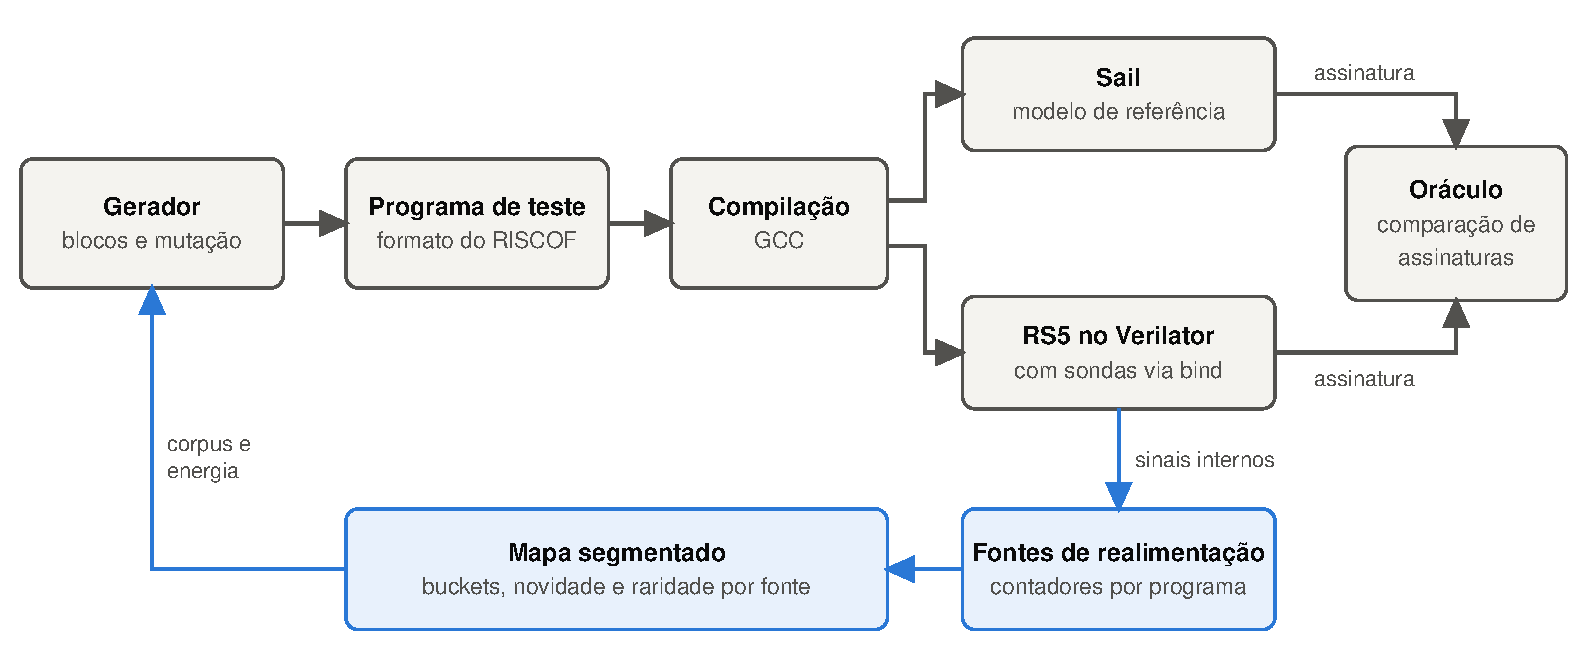
\includegraphics[width=\textwidth]{fig/fluxo_fuzzer.pdf}
    \caption{Fluxo de um programa no \textit{fuzzer}. Em azul, o laço de realimentação.}
    \label{fig:fluxo}
\end{figure}

Um programa é composto por um prólogo, que inicializa os registradores e uma região de memória, por três a oito blocos e por um epílogo, que grava os registradores na assinatura. Nesta versão preliminar os blocos são sintéticos e organizados por classe de instrução: operações lógicas e aritméticas, acessos à memória, multiplicação e divisão, desvios, laços, saltos e acessos a CSRs. Cada bloco favorece o uso de registradores escritos há pouco, para formar dependências entre instruções. O corpus de blocos extraídos de aplicações reais, previsto nos objetivos, substituirá esses blocos. As mutações atuam sobre blocos inteiros: substituição, inserção, remoção, troca de posição, recombinação entre dois programas e alteração dos valores iniciais. Quando há corpus, 80\% dos programas são mutações de um pai sorteado conforme sua energia, e os demais são gerados do zero.

Uma segunda versão do gerador acrescenta \textit{traps}. O programa passa a incluir um tratador que registra a causa na assinatura, avança sobre a instrução que a provocou e retorna. O gerador ganha três tipos de bloco: exceções (chamadas de sistema, instruções ilegais, escritas em CSRs somente de leitura e acessos desalinhados), interrupções de temporizador habilitadas em torno de uma a três instruções, e trechos executados em modo de usuário. Valores que diferem legitimamente entre o RS5 e o Sail não chegam à assinatura, como os contadores de desempenho e o endereço de retorno de uma interrupção, que depende do ciclo em que ela é aceita.

As fontes são capturadas por módulos SystemVerilog ligados ao RS5 pela construção \texttt{bind}, sem alteração do RTL. Cada fonte ocupa uma região do mapa, com contadores gravados ao final da simulação, e o \textit{fuzzer} aplica a cada região a regra de \textit{buckets} e de novidade. Todas as fontes são registradas em todas as execuções; a linha de comando define quais delas decidem a entrada no corpus e a energia, e a geração sem realimentação é o mesmo \textit{fuzzer} com esse conjunto vazio. As sondas custam cerca de 1~ms por programa, 5\% do tempo de simulação, enquanto a instrumentação de cobertura do Verilator triplica esse tempo, de 18,5 para 54,9~ms.

\section{Experimentos}\label{sec:previo-exp}

Os experimentos usaram o RS5 na configuração RV32IM com Zicsr e Zihpm, modos de máquina e de usuário, predição de desvios e encaminhamento habilitados, fila de duas instruções e memória de dados com dois ciclos de latência, escolhida por ativar o \textit{stall}. Foram executados cerca de 1,8 milhão de programas em três campanhas: duas com rodadas de 8.000 programas, para comparar as fontes e os geradores, e uma com rodadas de 200.000 programas, para observar a saturação. Os grupos principais foram repetidos com três sementes. Entre as rodadas de uma comparação, o gerador e a semente são mantidos, e apenas a fonte que guia a exploração muda. O objetivo desses experimentos é comparar as fontes, e não avaliar o \textit{fuzzer} final: o gerador e as mutações utilizados são provisórios.

\subsection{Saturação das fontes}\label{sec:previo-sat}

A \cref{tab:saturacao} resume o comportamento de cada fonte sob geração aleatória com o gerador com \textit{traps}. As posições são os elementos distintos que a fonte registrou: pontos de cobertura, \textit{bins}, transições ou arestas.

\begin{table}[H]
    \centering
    \caption{Saturação das fontes em 200.000 programas aleatórios (três sementes). As colunas de 50\% e 90\% indicam quantos programas foram necessários para atingir essa fração do total observado.}
    \label{tab:saturacao}
    \small
    \begin{tabular}{|l|r|r|r|r|}
        \hline
        \textbf{Fonte} & \textbf{Posições} & \textbf{50\%} & \textbf{90\%} & \textbf{Novas nos últimos 10.000} \\
        \hline
        Cobertura do Verilator$^{*}$ & 1.052 & 2 a 4 & 61 a 64 & 0 \\
        \hline
        \textit{Bins} & 49 de 64 & 2 a 3 & 34 a 73 & 0 \\
        \hline
        Transições de CSRs & 978 $\pm$ 3 & 2.100 a 2.600 & 56.000 a 57.000 & 2 a 6 \\
        \hline
        Arestas do \textit{pipeline} & 30.736 $\pm$ 40 & 9.400 a 9.600 & 107.000 a 108.000 & 238 a 253 \\
        \hline
        \multicolumn{5}{l}{\footnotesize $^{*}$ Medida em rodadas de 8.000 programas, por causa do custo da instrumentação.}
    \end{tabular}
\end{table}

A cobertura do Verilator e os \textit{bins} esgotam-se em centenas de programas. A partir desse ponto todo programa repete o que já foi visto, e a fonte deixa de distinguir um programa de outro. Os 15 \textit{bins} restantes permaneceram em zero nos 600.000 programas das três sementes. As transições de CSRs formam um espaço de cerca de mil posições, quase todo observado ao fim das rodadas. As arestas do \textit{pipeline} são a única fonte que continua a crescer: ao fim de 200.000 programas ainda surgem cerca de 250 arestas novas a cada 10.000. O estimador Chao1 \citep{chao1984}, aplicado ao número de arestas vistas em um e em dois programas, indica cerca de 35 mil arestas alcançáveis por esse gerador, das quais 87\% foram observadas. As três sementes diferem em menos de 0,3\% no total, o que mostra que esses números são propriedade do gerador, e não do acaso.

\subsection{Geração aleatória e geração guiada}\label{sec:previo-guiada}

A \cref{fig:saturacao} compara quatro formas de gerar 200.000 programas. Nas duas primeiras não há realimentação, e o que muda é o gerador, sem e com \textit{traps}. Na terceira, as arestas do \textit{pipeline} guiam a exploração. A quarta isola o efeito do sinal: aplica as mesmas mutações, na mesma proporção, mas admite todo programa no corpus e sorteia os pais ao acaso.

\begin{figure}[htb]
    \centering
    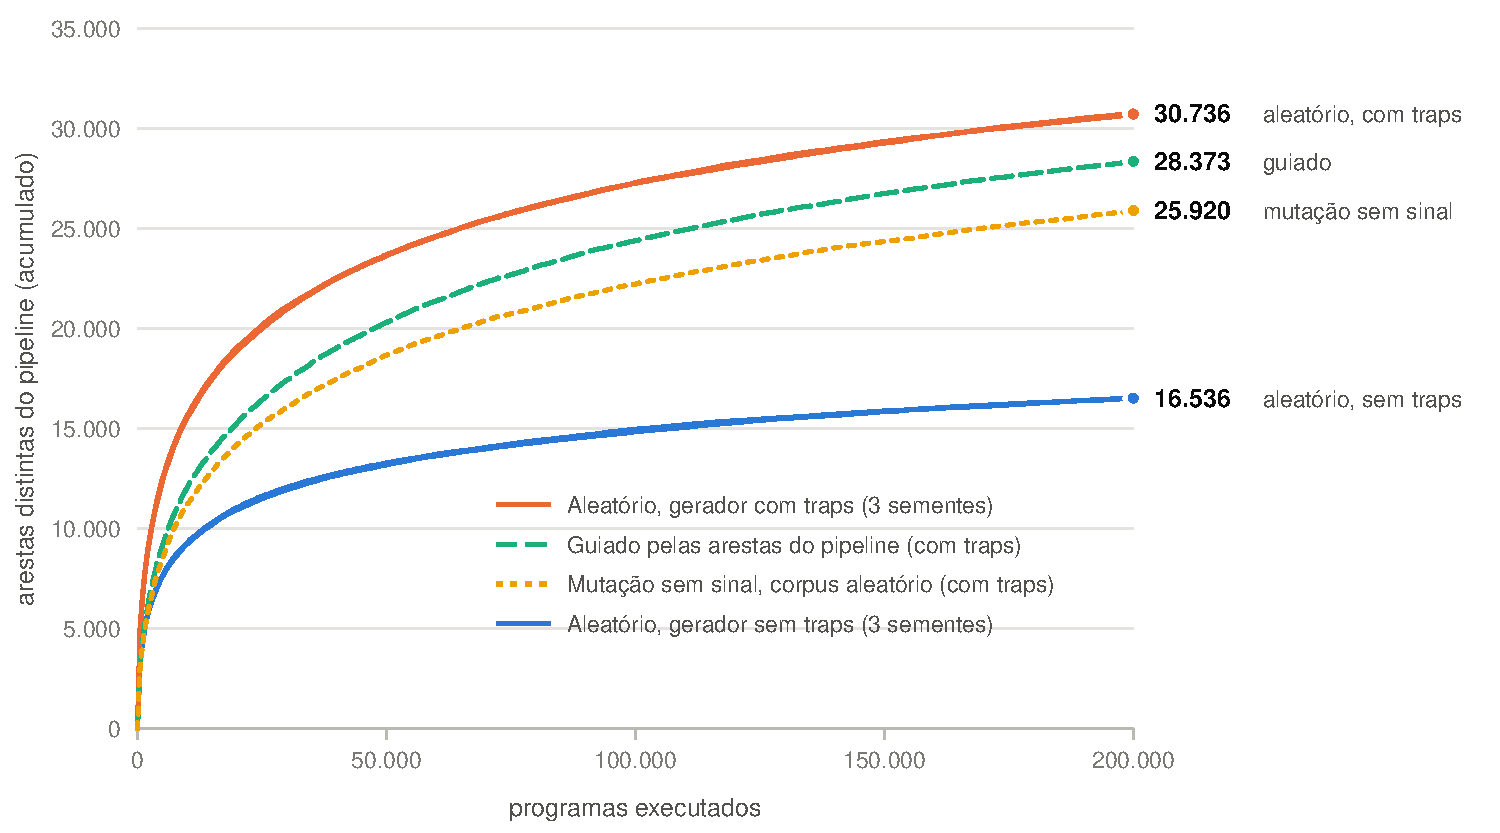
\includegraphics[width=\textwidth]{fig/saturacao_arestas.pdf}
    \caption{Arestas distintas do \textit{pipeline} acumuladas ao longo de 200.000 programas. As rodadas aleatórias têm três sementes cada, que se sobrepõem.}
    \label{fig:saturacao}
\end{figure}

Com 8.000 programas, a rodada guiada alcançou 76\% das arestas da aleatória (11.085 contra 14.573). A causa é a mutação, e não o sinal. Um programa gerado do zero trouxe em média 3,8 arestas novas, contra 0,2 a 1,2 de um programa mutado, e a perda cresceu na proporção dos programas mutados quando essa fração foi variada. Com o mesmo mutador, escolher os pais pelo sinal rendeu mais arestas do que escolhê-los ao acaso nas três sementes testadas.

A diferença para a geração aleatória diminui continuamente com o orçamento, como mostra a \cref{fig:razao}: a rodada guiada tem 66\% das arestas da aleatória com 1.000 programas, 76\% com 8.000, 86\% com 50.000 e 92\% com 200.000. Nos últimos 50.000 programas ela acrescentou 1.607 arestas, contra 1.388 a 1.427 das rodadas aleatórias. A vantagem do sinal sobre a mutação sem sinal também cresce, de 7\% para 9,5\%.

\begin{figure}[htb]
    \centering
    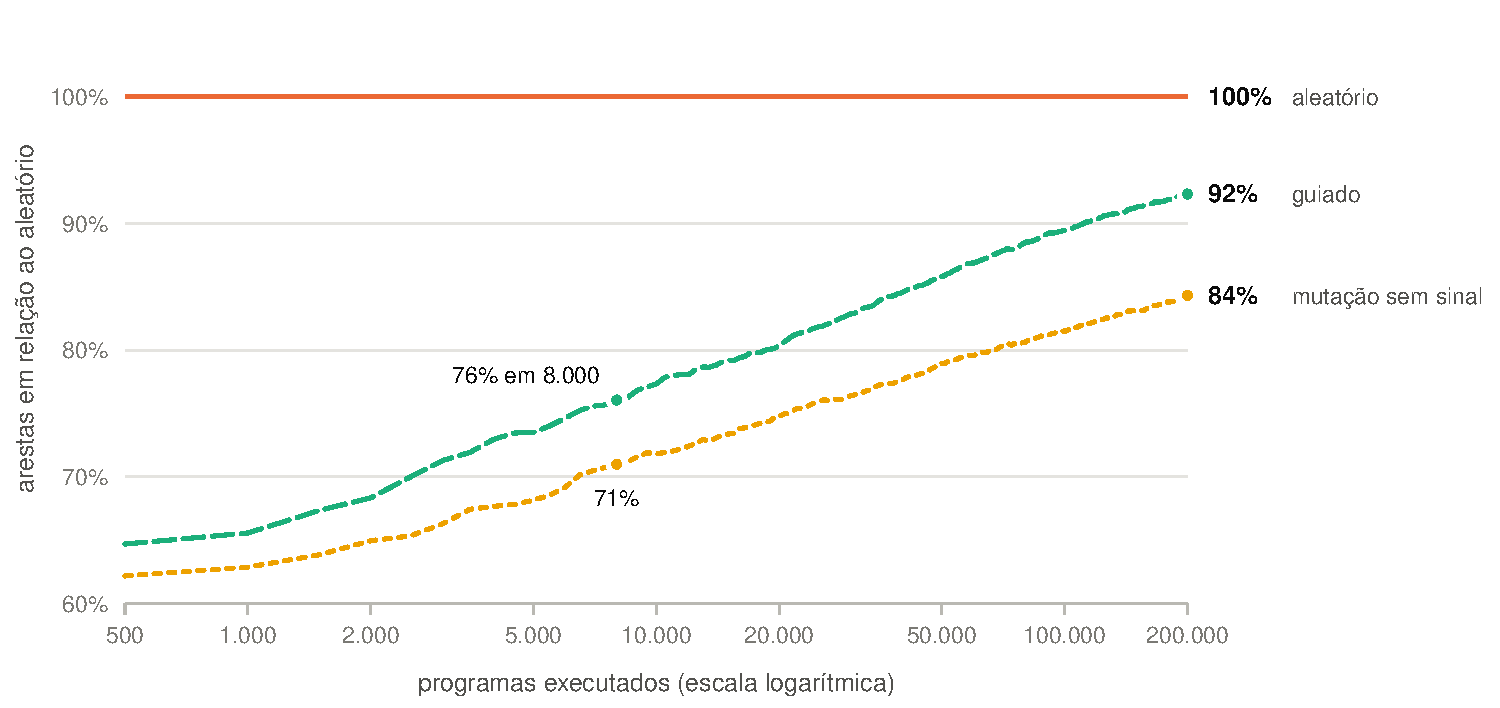
\includegraphics[width=\textwidth]{fig/razao_guiado.pdf}
    \caption{Arestas alcançadas com mutação, em relação à média das três rodadas aleatórias com o mesmo gerador.}
    \label{fig:razao}
\end{figure}

A realimentação muda sobretudo o tratamento dos estados raros. Na rodada aleatória, 16\% das arestas foram vistas em um único programa; na guiada, 5,6\%. Das 11.815 arestas que apareceram em no máximo cinco dos 200.000 programas de uma rodada aleatória, a rodada guiada alcançou 7.052 e exercitou cada uma em seis programas, na mediana, enquanto outra rodada aleatória alcançou 8.533, em dois programas cada. Em relação a 400.000 programas aleatórios, uma nova rodada aleatória contribui com 1.745 a 1.806 arestas inéditas, a rodada guiada com 1.603 a 1.729 e a mutação sem sinal com 629 a 850. Com 8.000 programas, a contribuição da rodada guiada era cerca de metade da de uma rodada aleatória (966 a 1.170 contra 2.007 a 2.067) e pouco superior à da mutação sem sinal. Portanto, dentro do orçamento medido, a rodada guiada não superou a aleatória no total de estados, e não há evidência de que ela alcance estados inacessíveis à geração aleatória. O que os dados mostram é que sua desvantagem inicial se reduz de forma contínua e que ela revisita os estados raros com mais frequência.

Duas características da infraestrutura preliminar explicam a vantagem da geração aleatória. A primeira é o mutador: como cada mutação preserva a maior parte do programa de origem, um programa mutado repete quase todos os estados do pai. A segunda é o espaço de estados produzido pelo gerador, que é raso. As arestas raras são, em sua maioria, combinações de características independentes, como a origem do encaminhamento, o nível da fila e a classe da instrução, e não situações que dependam de uma sequência anterior específica. Em um espaço assim, sortear programas novos cobre bem as combinações, e há pouco a ganhar em partir de um programa que já chegou a um estado raro.

Uma limitação dessas medidas é o tamanho do mapa: com $2^{16}$ posições, de 5\% a 8\% das posições das arestas sofreram colisão, o que subestima os totais de todas as rodadas. O mapa será ampliado nas próximas campanhas.

\subsection{Divergência encontrada}\label{sec:previo-bug}

Nenhum dos 80.000 programas sem \textit{traps} da segunda campanha divergiu do Sail. Com \textit{traps}, 354 de 80.000 divergiram, todos pela mesma causa. Quando um programa habilita a interrupção de temporizador, executa uma instrução e desabilita as interrupções com uma escrita em \texttt{mstatus}, o RS5 aceita a interrupção no ciclo em que essa escrita termina. A atualização de \texttt{mstatus} pela entrada no \textit{trap} tem prioridade sobre a escrita da instrução, que se perde: após o retorno, as interrupções estão habilitadas no RS5 e desabilitadas no Sail. A divergência foi reproduzida por um teste dirigido com oito variantes da sequência e não depende da latência da memória. Nas rodadas de 200.000 programas, ela foi disparada por 0,37\% a 0,40\% dos programas aleatórios.

A \cref{tab:bug} mostra quantos programas dispararam a divergência conforme a fonte que guiou a rodada.

\begin{table}[H]
    \centering
    \caption{Programas que dispararam a divergência em rodadas de 8.000 programas com o gerador com \textit{traps}.}
    \label{tab:bug}
    \small
    \begin{tabular}{|l|r|r|}
        \hline
        \textbf{Realimentação} & \textbf{Programas que dispararam} & \textbf{Programa do décimo disparo} \\
        \hline
        Nenhuma (três sementes) & 25, 30 e 33 & 2.424 a 3.388 \\
        \hline
        Arestas do \textit{pipeline} & 27 & 2.982 \\
        \hline
        Transições de CSRs & 131 & 756 \\
        \hline
        Mutação sem sinal & 14 & 5.517 \\
        \hline
    \end{tabular}
\end{table}

A rodada guiada pelas transições de CSRs disparou a divergência quatro vezes mais do que as aleatórias e chegou ao décimo disparo bem antes delas. A rodada guiada pelas arestas do \textit{pipeline} não se distinguiu da geração aleatória. Trata-se de uma única falha, mas o resultado indica que a fonte que acumula mais estados não é necessariamente a que mais dispara uma falha: a métrica de CSRs distingue exatamente os estados em que essa falha se manifesta.

\section{Considerações}\label{sec:previo-remarks}

O resultado mais nítido é o peso do gerador. Acrescentar \textit{traps} ampliou as arestas observadas em 86\% (de 16.536 para 30.736), as transições de CSRs de 584 para 978 e os \textit{bins} atingidos de 31 para 49, e somente os programas com \textit{traps} revelaram a divergência. Nenhuma fonte de realimentação produziu efeito comparável, e nenhuma quantidade de programas alcançou os \textit{bins} que o gerador não sabe produzir. Isso está de acordo com o Encarsia, segundo o qual os programas gerados determinam quais falhas são encontradas, mais do que o mecanismo de realimentação.

Os \textit{traps} importam também pelo que exercitam. Exceções, interrupções e retornos são o caminho pelo qual o processador muda de modo de privilégio, e a separação entre os modos de máquina e de usuário depende de que esse estado seja atualizado corretamente. A divergência encontrada pertence a essa classe: um programa que desabilita as interrupções para proteger uma região crítica prossegue com elas habilitadas. Como observa o Encarsia, toda falha arquiteturalmente observável pode ter implicações de segurança, e as falhas no estado privilegiado são as de consequência mais direta.

Quanto às fontes, as arestas do \textit{pipeline} serão a fonte principal do \textit{fuzzer}: é a única que não se esgota, mantém resolução para distinguir programas ao longo de toda a campanha e corresponde à realimentação funcional que o Encarsia recomenda. As transições de CSRs serão usadas como fonte complementar. Seu espaço é pequeno, mas ela favoreceu a única falha encontrada, o que é coerente com a proposta do ProcessorFuzz nesse caso e não contradiz o Encarsia, cujo resultado se refere a conjuntos de falhas distribuídas pelo projeto. A cobertura do Verilator fica restrita ao relato dos resultados, e os \textit{bins}, ao diagnóstico do gerador.

Os experimentos deste capítulo não avaliam o \textit{fuzzer} proposto: são um estudo da saturação das fontes, feito com um gerador e um mutador provisórios. Nesse cenário a exploração guiada ficou abaixo da geração aleatória no total de estados, pelas duas limitações apontadas na \cref{sec:previo-guiada}. Ambas pertencem ao gerador, e não ao sinal, e a tendência medida é favorável: a desvantagem cai de 34\% para 8\% entre 1.000 e 200.000 programas, e a escolha dos pais pelo sinal supera a escolha ao acaso em todos os orçamentos. Por isso, a proposta para a continuidade do trabalho é melhorar o gerador e a mutação até que a exploração guiada supere a geração aleatória nos estados alcançados. Espera-se que o corpus de blocos extraídos de aplicações reais aprofunde o espaço de estados, por trazer cadeias de dependência mais longas entre as instruções, e os operadores de mutação passarão a alterar mais de um bloco, para que um programa mutado se afaste mais de sua origem. A hipótese é que, em um espaço mais profundo, partir dos programas que alcançaram estados raros renda mais do que sortear programas novos.

O número de estados, porém, é uma medida intermediária: o que se quer do \textit{fuzzer} são falhas encontradas, e até aqui há uma única divergência para sustentar qualquer conclusão nesse sentido. A resposta também depende do orçamento, pois com 8.000 programas a realimentação parece prejudicial e só em campanhas longas sua desvantagem se reduz. O \textit{fuzzer} final será avaliado pelo tempo até a detecção de falhas injetadas no RS5, uma por vez, como propõe o Encarsia, com curvas ao longo do orçamento em lugar de um único ponto e com a geração aleatória como linha de base em todas as comparações.


% ---------------------------------------------------------------------------
% Roteiro original do capítulo (mantido como referência)
% ---------------------------------------------------------------------------
% \chapter{Trabalho previo - sugerir titulo para o capitulo}
% 
% - Levantamento de sinais para servir como feedback do fuzzer
%     * Random -> usado como baseline
%     * Coverage do SystemVerilog
%     * Estado do pipeline -> OK, apontar para seção que vai detalhar os experimentos
%         -> Como é um core pequeno, diferencial que pode mapear o pipeline
%     * CSRs (valores contidos neles)
%         -> Relacionar ProcessorFuzz com Encarsia - um é oposto do outro, ref com a seção de experimentos
%     * Bins (propriedades relacionadas entre sinais/registradores) -> justificar por que não foi usado
%         -> Dá hints da microarquitetura - não é o que procuramos aqui
%         -> Da muito vies do programador (tentar achar uma referencia aqui)
% 
% - Descrever como foi implementado o fuzzer e como ele funciona em conjunto com o RISCOF
% 
% - Descrição dos experimentos e resultados
%     * Random vs. guided - experimentos
%     * Gráficos
%     * Resultados
%     * Falar que com 8000 testes o guided perdeu para o random em estados totais, mas com mais testes ele ganha (o guided consegue achar estados raros, enquanto o random nao, por isso ele ultrapassa)
% 
% - Seção final de 'remarks'
%     * Gerador com traps -- Encarsia cita que o gerador é mais importante (tao importante quanto) o feedback - segue o que foi encontrado
%         -> É importante a parte de traps devido ao teste de privilégios (modos) de execução - bug é falha de segurança!!!!!

\chapter{\label{chap:cronograma}Cronograma}

Este capítulo apresenta as atividades previstas para o primeiro semestre de 2027 e as relaciona aos objetivos específicos definidos no \cref{chap:intro}. A \cref{sec:crono-objetivos} avalia a situação de cada objetivo a partir do trabalho descrito no \cref{chap:previo}, e a \cref{sec:crono-atividades} apresenta o cronograma e descreve as atividades.

\section{Situação dos objetivos}\label{sec:crono-objetivos}

Três objetivos já foram atingidos e, por isso, não aparecem no cronograma.

\begin{itemize}
    \item O \cref{obj:1} foi atingido pela infraestrutura da \cref{sec:previo-impl}. Cada programa gerado é um teste no formato do RISCOF, compilado com as mesmas ferramentas e executado no RS5 e no Sail, e as assinaturas são comparadas. A alteração que passou a compilar o modelo uma única vez foi incorporada ao repositório do RS5.

    \item O \cref{obj:5} foi atingido pela integração da cobertura do Verilator como uma das fontes de realimentação (\cref{sec:previo-fontes}). Ela é coletada a cada programa e pode decidir a entrada no corpus. Os experimentos da \cref{sec:previo-sat} mostraram que essa cobertura se esgota em centenas de programas, o que definiu o seu papel: critério complementar de avaliação, e não a fonte principal de seleção.

    \item O \cref{obj:8} foi atingido pelo oráculo do \textit{fuzzer}. Todo programa cuja assinatura difere da produzida pelo Sail é salvo com os arquivos necessários para reproduzi-lo, na forma de um teste do RISCOF. O mecanismo já revelou uma divergência no RS5, reproduzida por um teste dirigido (\cref{sec:previo-bug}).
\end{itemize}

Quatro objetivos foram atingidos em parte, e o cronograma cobre o que falta. Para o \cref{obj:3}, o gerador já combina blocos e os modifica com seis operadores (\cref{sec:previo-gerador-mutacao}), mas todos atuam sobre blocos inteiros; faltam as mutações internas ao bloco. Para o \cref{obj:4}, o mapa de realimentação, a regra de novidade e a energia estão implementados, e as fontes que orientarão a exploração foram escolhidas (\cref{sec:previo-remarks}), mas a decisão entre gerar um programa e mutar um existente ainda é uma proporção fixa. Para o \cref{obj:6}, o \textit{fuzzer} recebe a descrição da ISA e os parâmetros da microarquitetura e compila o modelo correspondente, mas a execução sobre um conjunto de configurações não está automatizada. Para o \cref{obj:9}, os experimentos da \cref{sec:previo-exp} são uma avaliação preliminar, restrita às fontes de realimentação.

Os \cref{obj:2,obj:7} não foram iniciados: os blocos atuais são sintéticos, e todas as campanhas usaram uma única configuração do processador.

\section{Atividades}\label{sec:crono-atividades}

A \cref{fig:cronograma} distribui as atividades ao longo do semestre. A lista que a segue descreve cada atividade, os objetivos que ela cumpre e o resultado esperado.

\begin{figure}[htbp]
    \centering
    \begin{ganttchart}[
        x unit=1.05cm,
        y unit title=0.65cm,
        y unit chart=0.62cm,
        vgrid={*1{black!15, dashed}},
        hgrid={*1{black!8}},
        title/.style={draw=none, fill=none},
        title label font=\small\bfseries,
        title height=1,
        bar/.style={draw=none, fill=ganttBar, rounded corners=1.5pt},
        bar height=0.55,
        bar top shift=0.225,
        bar label font=\small,
        bar label node/.append style={align=left, text width=8.2cm, xshift=-6pt},
        canvas/.style={draw=black!25},
    ]{1}{6}
        \gantttitle{Jan}{1} \gantttitle{Fev}{1} \gantttitle{Mar}{1}
        \gantttitle{Abr}{1} \gantttitle{Mai}{1} \gantttitle{Jun}{1} \\
        \ganttbar{\ref{atv:corpus}\quad Corpus de blocos de aplicações reais}{1}{2} \\
        \ganttbar{\ref{atv:mutacao}\quad Mutação e composição dos blocos}{2}{3} \\
        \ganttbar{\ref{atv:criterio}\quad Critério de mutação}{3}{4} \\
        \ganttbar{\ref{atv:config}\quad Automação das configurações}{3}{3} \\
        \ganttbar{\ref{atv:falhas}\quad Falhas injetadas para a avaliação}{4}{4} \\
        \ganttbar{\ref{atv:campanhas}\quad Campanhas em diferentes configurações}{4}{5} \\
        \ganttbar{\ref{atv:avaliacao}\quad Avaliação da abordagem}{5}{6} \\
        \ganttbar{\ref{atv:redacao}\quad Redação do volume final}{5}{6}
    \end{ganttchart}
    \caption{Cronograma das atividades para o primeiro semestre de 2027.}
    \label{fig:cronograma}
\end{figure}

\begin{atividades}
    \item \label{atv:corpus} \textbf{Corpus de blocos de aplicações reais.} Selecionar aplicações que contenham os padrões computacionais citados na introdução, como reduções, transformações de elementos, produtos escalares e operações matriciais, compilá-las para a ISA do RS5 e extrair blocos delimitados por transferências de controle, com a anotação dos registradores e das regiões de memória que cada bloco usa. Cumpre o \cref{obj:2}. Resultado esperado: um corpus de blocos integrado ao gerador, em substituição aos blocos sintéticos.

    \item \label{atv:mutacao} \textbf{Mutação e composição dos blocos.} Implementar os operadores que atuam dentro do bloco, com substituição de registradores, alteração de operandos, reordenação de instruções e modificação das dependências, preservada a estrutura de controle. Implementar também os operadores que alteram mais de um bloco e as composições que o gerador atual não produz (\cref{sec:previo-gerador-planos}). Completa o \cref{obj:3}. Resultado esperado: programas mutados que tragam mais estados novos do que os da versão atual, medidos em arestas novas por programa nas condições da \cref{sec:previo-guiada}.

    \item \label{atv:criterio} \textbf{Critério de mutação.} Substituir a proporção fixa de mutações por um critério que acompanhe o rendimento medido de cada origem e de cada operador, com as arestas do \textit{pipeline} como fonte principal e as transições de CSRs como fonte complementar, e ampliar o mapa das arestas. Completa o \cref{obj:4}. Resultado esperado: uma exploração guiada que alcance, com o mesmo número de programas, ao menos tantos estados quanto a geração aleatória.

    \item \label{atv:config} \textbf{Automação das configurações.} Construir o mecanismo que executa uma campanha sobre uma lista de configurações. Para cada combinação de descrição da ISA e de parâmetros da microarquitetura (encaminhamento, predição de desvios, tamanho da fila de instruções, organização e latência da memória), ele compila um modelo, executa os programas e reúne os resultados. Completa o \cref{obj:6}. Resultado esperado: uma campanha sobre várias configurações disparada por um único comando, com as divergências identificadas por configuração.

    \item \label{atv:falhas} \textbf{Falhas injetadas para a avaliação.} Preparar o conjunto de falhas usado na avaliação: alterações no RTL do RS5 dos dois tipos identificados pelo Encarsia, trocas de sinais e condicionais incorretas, cada uma acompanhada de um teste dirigido que comprove que ela é observável na assinatura. Cumpre em parte o \cref{obj:9}. Resultado esperado: um conjunto de versões do RS5 com uma falha cada, distribuídas pelos módulos do processador.

    \item \label{atv:campanhas} \textbf{Campanhas em diferentes configurações.} Executar o \textit{fuzzer} nas configurações preparadas na \cref{atv:config}, variando as extensões suportadas pelo gerador, a política de encaminhamento, o tamanho da fila de instruções, a organização da memória e a sua latência. Cumpre o \cref{obj:7}. Resultado esperado: para cada configuração, os estados alcançados e as divergências encontradas. As divergências confirmadas serão relatadas no repositório do RS5.

    \item \label{atv:avaliacao} \textbf{Avaliação da abordagem.} Comparar a exploração guiada com a geração aleatória, e as fontes de realimentação entre si, pelo tempo até a detecção das falhas da \cref{atv:falhas}, com várias sementes e curvas ao longo do orçamento. Comparar também a cobertura e os estados alcançados com os das suítes \textit{riscv-tests} e do RISCOF. Completa o \cref{obj:9}. Resultado esperado: evidência, favorável ou não, de que a realimentação escolhida encontra falhas antes da geração aleatória, e a relação dos comportamentos que as suítes existentes não exercitam.

    \item \label{atv:redacao} \textbf{Redação do volume final.} Escrever o volume do Trabalho de Conclusão II com os resultados das atividades anteriores e preparar a defesa. Não corresponde a um objetivo específico. Resultado esperado: o volume final.
\end{atividades}


%----------------------------------------------------------------
% Aqui vai a bibliografia. Existem 3 estilos de citação: use
% 'tcc-alpha' para citações do tipo [Abc+] ou [XYZ] (em ordem
% alfabética na bibliografia), 'tcc-num' para citações
% numéricas do tipo [1], [20], etc., em ordem de referência e
% 'tcc-alpha-full' para citações estilo 'alpha' mas com nomes completos.
%----------------------------------------------------------------
\bibliographystyle{apalike}
%\bibliographystyle{tcc-num}
\bibliography{tcc}

%----------------------------------------------------------------
% Após \appendix, se iniciam os capítulos de Apêndice, com
% numeração alfabética.
%----------------------------------------------------------------
% \appendix
% \chapter{Meu primeiro apêndice}
% \chapter{My second appendix}

%----------------------------------------------------------------
% Aqui vão os "capítulos" de anexos. Cada anexo deve
% ser considerado um capítulo.
%----------------------------------------------------------------
% \anexos
% \chapter{Meu primeiro anexo}
% \chapter{My second attachment}

% E aqui (para a felicidade de todos) termina o documento.
\end{document}
